\documentclass[english,DIV=13]{scrreprt}
%\documentclass[english,DIV=13]{scrartcl}

\usepackage[utf8x]{inputenc}
\usepackage[T1]{fontenc}
\usepackage{lmodern}
\usepackage[binary-units=true]{siunitx}
% Color
% cfr http://en.wikibooks.org/wiki/LaTeX/Colors
\usepackage{color}
\usepackage[usenames,dvipsnames,svgnames,table]{xcolor}
\definecolor{dkgreen}{rgb}{0.25,0.7,0.35}
\definecolor{dkred}{rgb}{0.7,0,0}
\usepackage{graphicx}
\usepackage{url}
\usepackage{tikz}
\usepackage{pgfplots}
\usepackage{microtype}
\usepackage{xspace}

\usepackage{hyperref}
\usepackage{todonotes}
\usepackage{epstopdf}

\usepackage{multirow}
\usepackage{tabularx} % tabular with automatic line-break
\newcolumntype{Y}{>{\centering\arraybackslash}X} % centered column

\newcommand{\matlab}{\textsc{Matlab}}

% Math symbols
\usepackage{amsmath}
\usepackage{amssymb}
\usepackage{amsthm}
\DeclareMathOperator*{\argmin}{arg\,min}
\DeclareMathOperator*{\argmax}{arg\,max}

% Unit vectors
\usepackage{esint}
\usepackage{esvect}
\newcommand{\kmath}{k}
\newcommand{\xunit}{\hat{\imath}}
\newcommand{\yunit}{\hat{\jmath}}
\newcommand{\zunit}{\hat{\kmath}}
\newcommand{\uunit}{\hat{\umath}}

% Elec
\newcommand{\B}{\vec B}
\newcommand{\E}{\vec E}
\newcommand{\EMF}{\mathcal{E}}
\newcommand{\perm}{\varepsilon} % permittivity

\newcommand{\bigoh}{\mathcal{O}}
\newcommand\eqdef{\triangleq}

\DeclareMathOperator{\newdiff}{d} % use \dif instead
\newcommand{\dif}{\newdiff\!}
\newcommand{\fpart}[2]{\frac{\partial #1}{\partial #2}}
\newcommand{\ffpart}[2]{\frac{\partial^2 #1}{\partial #2^2}}
\newcommand{\fdpart}[3]{\frac{\partial^2 #1}{\partial #2\partial #3}}
\newcommand{\fdif}[2]{\frac{\dif #1}{\dif #2}}
\newcommand{\ffdif}[2]{\frac{\dif^2 #1}{\dif #2^2}}
\newcommand{\constant}{\ensuremath{\mathrm{cst}}}
\newcommand{\norm}[1]{\left\lVert#1\right\rVert}

\usepackage{babel}
% Listing
% always put it after babel
% http://tex.stackexchange.com/questions/100717/code-in-lstlisting-breaks-document-compile-error
\usepackage{listings}

% Put caption after babel
\usepackage{caption}
\usepackage{subcaption}

\definecolor{mygreen}{rgb}{0,0.6,0}
\definecolor{mygray}{rgb}{0.5,0.5,0.5}
\definecolor{mymauve}{rgb}{0.58,0,0.82}
\lstset{ %
  language=Matlab,
  backgroundcolor=\color{white},   % choose the background color; you must add \usepackage{color} or \usepackage{xcolor}
  basicstyle=\footnotesize,        % the size of the fonts that are used for the code
  breakatwhitespace=false,         % sets if automatic breaks should only happen at whitespace
  breaklines=true,                 % sets automatic line breaking
  captionpos=b,                    % sets the caption-position to bottom
  commentstyle=\color{mygreen},    % comment style
  deletekeywords={...},            % if you want to delete keywords from the given language
  escapeinside={\%*}{*)},          % if you want to add LaTeX within your code
  extendedchars=true,              % lets you use non-ASCII characters; for 8-bits encodings only, does not work with UTF-8
  frame=single,	                   % adds a frame around the code
  keepspaces=true,                 % keeps spaces in text, useful for keeping indentation of code (possibly needs columns=flexible)
  keywordstyle=\color{blue},       % keyword style
  otherkeywords={*,...},           % if you want to add more keywords to the set
  numbers=none,                    % where to put the line-numbers; possible values are (none, left, right)
  numbersep=5pt,                   % how far the line-numbers are from the code
  numberstyle=\tiny\color{mygray}, % the style that is used for the line-numbers
  rulecolor=\color{black},         % if not set, the frame-color may be changed on line-breaks within not-black text (e.g. comments (green here))
  showspaces=false,                % show spaces everywhere adding particular underscores; it overrides 'showstringspaces'
  showstringspaces=false,          % underline spaces within strings only
  showtabs=false,                  % show tabs within strings adding particular underscores
  stepnumber=2,                    % the step between two line-numbers. If it's 1, each line will be numbered
  stringstyle=\color{mymauve},     % string literal style
  tabsize=2,	                   % sets default tabsize to 2 spaces
  title=\lstname                   % show the filename of files included with \lstinputlisting; also try caption instead of title
}

\KOMAoptions{DIV=last}




% Definition to put a bar under a letter/word (to use with matrix)
\usepackage{accents}
\newcommand{\ubar}[1]{\underaccent{\bar}{#1}}
\newcommand{\uvec}[1]{\ubar{#1}}
\newcommand{\umatrix}[1]{\ubar{\ubar{#1}}}

\titlehead{}
\subject{LINMA 1731 --- Stochastic processes}
\title{Bearings-only tracking problem}
\subtitle{}
\author{\begin{tabular}{cc}
	\textsc{Cassiers} Gaëtan  & 	$33741300$ \\
	\textsc{Losseau} Bruno 	&	$33741300$
	 \end{tabular}}
\date{\today}
\publishers{}

\begin{document}
\maketitle


\tableofcontents


%Q1
\chapter{Basics}
\section*{Deriving $\umatrix{F}$ and $\uvec{U}$}

We start by studying the making a discretization of a movemement process in 1D, with the
variable $x(t)$. If we denote $x_k = x(Tk)$ (with $T$ a given discretization step), we
get
\begin{align*}
    x_{k+1} &= x_k + T\dot{x}_k + \int_{Tk}^{T(k+1)}\int_{Tk}^{t}\ddot{x}(t)\dif t\dif t' \\
    \dot{x}_{k+1} &=  \dot{x}_k + \int_{Tk}^{T(k+1)}\ddot{x}(t)\dif t.
\end{align*}
This is a simple discrete-time state model, if we consider that the terms which depends of
the integral of $\ddot{x}$
are an input signal.
We can generalize this equation to the relative state vector $\uvec{x} = \uvec{x}^t - \uvec{x}^o$:
\[\uvec{x}_{k+1} = \umatrix{F}\uvec{x}_k - \uvec{U}_{k,k+1} + \uvec{\epsilon}_k\]
with
\begin{itemize}
    \item The matrix
        \[\umatrix{F} =
        \begin{pmatrix}
            1 & 0 & T & 0 \\
            0 & 1 & 0 & T \\   
            0 & 0 & 1 & 0 \\
            0 & 0 & 0 & 1   
        \end{pmatrix}
        \]
    \item $\uvec{\epsilon}_k$ the variation of position and of velocity of the target caused by the
acceleration of the target,
    \item $\uvec{U}_{k,k+1}$ the variation of position and velocity of
the observer caused by the acceleration of the observer.
\end{itemize}

\section*{Deriving $h(\ubar{x})$}
Following its definition given in the statement and using the notation $\uvec{x}(i)$
for the $i$-th element of the vector $\uvec{x}$:
\begin{align*}
    h(\uvec{x}_k) &= \mathrm{atan2}(\uvec{x}_k(1), \uvec{x}_k(2)) \\
    &= \begin{cases}
        \arctan\frac{\uvec{x}_k(1)}{\uvec{x}_k(2)} & \text{if $\uvec{x}_k(2) > 0$} \\
        \arctan\frac{\uvec{x}_k(1)}{\uvec{x}_k(2)}+\pi & \text{if $\uvec{x}_k(2) < 0$ and $\uvec{x}_k(1) \geq 0$} \\
        \arctan\frac{\uvec{x}_k(1)}{\uvec{x}_k(2)}-\pi & \text{if $\uvec{x}_k(2) < 0$ and $\uvec{x}_k(1) < 0$} \\
        0 & \text{if $\uvec{x}_k(2) \geq 0$ and $\uvec{x}_k(1) = 0$} \\
        \pi & \text{if $\uvec{x}_k(2) < 0$ and $\uvec{x}_k(1) = 0$}
    \end{cases}
\end{align*}

%Q2
\chapter{Simple model}
At first, without implementing any command, it is asked to simulate the system for $k=200$ steps, changing
the values of the variance $\sigma^2_{\theta}$ of the gausian noise on the bearing $w_k$  and
the variance  $\sigma^2_a$ of the gausian noise on the acceleration $\epsilon_k$.

\section*{Code}
For each chapter, one only presents the code that is strictly relevant. The scripts and functions 
used to plot the required results (herein \texttt{plot\_q2.m} and \texttt{gen\_plot2.m})
can be found in the linked archive. To obtain the results for all the questions, simply launch
the script \texttt{main.m}.\\

\lstinputlisting[caption={Simulating the system}]{../matlab/q2.m}

Every time a code uses a parameter given in the statement, it calls the following function : 
\lstinputlisting[caption={Parameters given in the statement}]{../matlab/gen_parameters.m}

\section*{Results}
\begin{itemize}
\item varying $\sigma_\theta$ with $\sigma_a=0$
\begin{center}	
\includegraphics[width=0.66\textwidth]{img/q2_1.eps}
\end{center}
When there is no noise, one verifies that as the relative velocity is constant and there is no error on
the bearing, the angle is constant and the the relative position is linear.\\
As the acceleration is by default equal to zero and that there is no noise on the acceleration, as the velocity is
constant, the trajectory is for all $\sigma_{\theta}$ the same.\\
Concerning the angle, the more we raise $\sigma_{\theta}$ the higher the error on the mesured angle is.

\item varying $\sigma_a$ with $\sigma_\theta=0$
\begin{center}
\includegraphics[width=0.66\textwidth]{img/q2_2.eps}
\end{center}
The more the noise on the acceleration increases, the more the trajectory is impacted. \\
In this case, the bearing is also impacted, it seems logical as one has changed the state equations :
the noise on the acceleration does change the relative position, therefore modyfing the true bearing. \\
From these comments, one could explain the situation stating that $\sigma_a$ represents the change of 
acceleration of the target, that can not be predicted. The change of acceleration induces a change
of position, therefrom a change on the bearing.


\item varying $\sigma_\theta$ proportionaly to $\sigma_a$
\begin{center}
\includegraphics[width=0.66\textwidth]{img/q2_3.eps}
\end{center}
The higher $\sigma_a$ is set, the quicker the relative distance augments. Taking a look at the bearing,
        we observe two trends: a slow (low frequency) variation, due to the acceleration of the target
         (which is integrated twice to get the bearing, therefore the variations are slow), and 
         a high frequency variation due to the measurement errors (that are adding a white noise).

\item  Keeping $\sigma_\theta$ and $\sigma_a$ constant

\begin{center}
 \includegraphics[width=0.66\textwidth]{img/q2_4.eps}
\end{center}
When $\sigma_a=0.5$ we observe that the target motion changes reasonably slowly, and
with $\sigma_{\theta}=0.1$ the mesurement noise is not adding too much uncertainty on the bearing. \\
With three simulations, one observes the randomness of the process.
\end{itemize}



%Q3
\chapter{Building a sequential Monte Carlo algorithm}
\section*{Code}
For all the methods that use a Monte Carlo algorithm, one built a general function 
\texttt{particle\_filter.m}, based on the reference document given in the statement
\footnote{A. Srivastava. Computational methods in statistics. Florida State University, 2009.
\url{http://stat.fsu.edu/~anuj/pdf/classes/CompStatII10/BOOK.pdf}}.\\
\lstinputlisting[caption={General Monte Carlo algorithm},label={MonteCarlo}]{../matlab/particle_filter.m}
The main code used here is the function \texttt{q3.m} (to employ it with the proper
parameters, plot and save the results one can launch the script \texttt{plot\_q3.m}).
\newpage
\lstinputlisting[caption={Comparing the results with Monte Carlo algorithm and the model}]{../matlab/q3.m}
\section*{Results}
By ploting the histograms of the distribution of the points used in the Monte Carlo algorithm, 
with $\sigma_a=0.1$ and $\sigma_{\theta}=0.1$, at the beginning (k=1) one has a look alike gaussian
distibution for both the X position and Y position. The more k augments, the less the
distribution looks like a gaussian and the wider is its variance (1 when k=1, to 50 for k=200).
This indicates that the quality of the estimation decreases when $k$ augments.

\begin{center}
   \includegraphics[width=0.49\textwidth]{img/q3_hist_1.eps}
   \includegraphics[width=0.49\textwidth]{img/q3_hist_50.eps}
   \includegraphics[width=0.49\textwidth]{img/q3_hist_100.eps}
   \includegraphics[width=0.49\textwidth]{img/q3_hist_200.eps}
\end{center}


\begin{center}
	\begin{minipage}{.6\textwidth}
		\includegraphics[width=0.95\textwidth]{img/q3_path.eps}
	\end{minipage}%
	\begin{minipage}{.4\textwidth}
		Plotting the real vs. the estimated position and indicating with dots the (X,Y) of the 
		herein produced histograms (k=1,50,100,200), one sees that the more $k$ augments
		the further the estimation is from the real position. The bearing is measured at each step (with a small error) and
		one can check that the result on the angle is convincing. Yet concerning the distance the measures don't bring
		much relevant information. What helps the best is the variability of the bearing, yet it is not enough. For this
		reason the distance is quite approximative.
	\end{minipage}
\end{center}

%Q4
\chapter{Applying the Monte Carlo algorithm to an artificial submarine 
tracking problem}
\section*{Code}

As the fourth and fifth questions are both established on applying the algorithm~\ref{MonteCarlo}
to the submarine tracking problem, one decided to group the main code for questions 4 and 5
in the function \texttt{q4q5.m}.\\
\lstinputlisting[caption={The artificial submarine tracking problem initialised with 'data.m'},label={q4q5}]{../matlab/q4q5.m}
To call \texttt{q4q5} in the present case, one should use \texttt{q4.m} (to use it with the proper parameters,
plot and save the results one can launch the script \texttt{plot\_q4.m}).\\
\lstinputlisting[caption={Question 4}]{../matlab/q4.m}

\section*{Results}
To introduce the results, one uses the following legends\\

	\begin{minipage}{.5\textwidth}
		\flushleft For the positions :\\
		 \center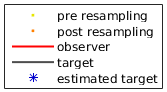
\includegraphics[width=4cm]{img/q4_legend1.png}
	\end{minipage}%
	\begin{minipage}{.3\textwidth}
		For the velocities :\\
		 \center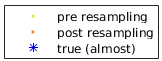
\includegraphics[width=4cm]{img/q4_legend2.png}
	\end{minipage}

\begin{itemize}
\item $k=1$\\
The distribution of the speed particles corresponds to the initial distribution ($k=0$) : as one doesn't have yet 2 measures 
of position of the target, it cannot estimate properly 
Concerning the cloud of position particles, as one doesn't know the distance but only the bearing, it forms a shape
that is close to a line. One can easily check by extending the "line" to the initial position of the observer that it 
follows the bearing.



\item The position\\
At the first step, the pre and post resampling clouds of points are forming a line, almost
the same. The center of gravity of the post resampling cloud is the estimated position
of the target.\\
At the second step, the pre resampling cloud forms a circle (distorted on the graph). 
The post resampling forms a line that estimates well the position of the target.\\
At the third step, the clouds seem to be already more concentrated around
the estimated positions. One can worry about the diversity of the points.\\
When $k=15$, the clouds form a line. They seem to be concentrated one
on top of the other. When one looks at the estimated position, the result
is not convincing. \\
In the end, even though one has some trouble with the predictions, the result
when $k=26$ is not much far from the real position.\\
One can wonder why such an error on the trajectory was not predicted in
section 3.

\item The velocitie\\
At the begining, one has a nice variety of points for the pre and post
resampling, they are (almost) all located in a circle of radius 1.
When k=2, the area where are located the pre resampling points is wide whilst
the area where are found the post resampling points is very narrow. From there, 
this area keeps narrowing. When k=26, the radius of the circle is only 0.03.

\item Conclusion\\
The results could be considered all right yet Monte Carlo method is loosing all its interest
for its core element (the generated cloud of points) is quickly loosing its
consistancy. One will improve the method in the next question!
\end{itemize} 


\begin{center}
	\begin{minipage}{.5\textwidth}
		 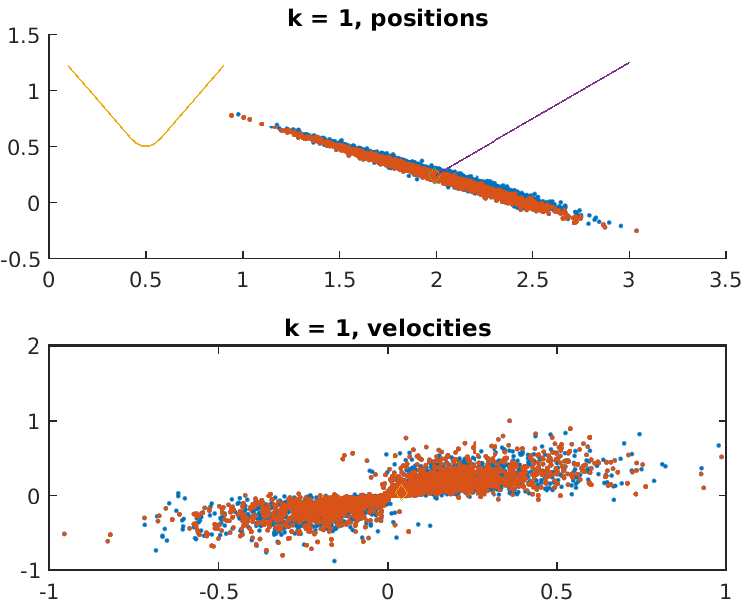
\includegraphics[width=.98\textwidth]{img/q4_1.png}
	\end{minipage}%
	\begin{minipage}{.5\textwidth}
		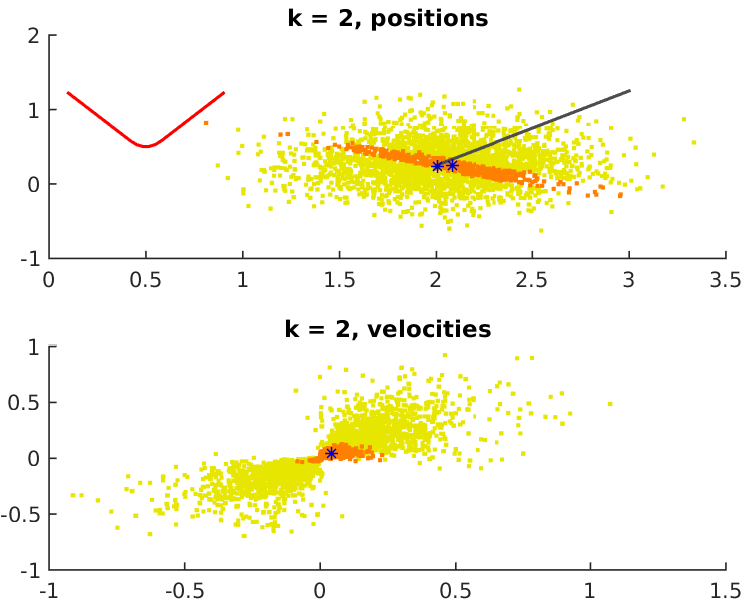
\includegraphics[width=0.98\textwidth]{img/q4_2.png}
	\end{minipage}
\end{center}
  \begin{center}
	\begin{minipage}{.5\textwidth}
   		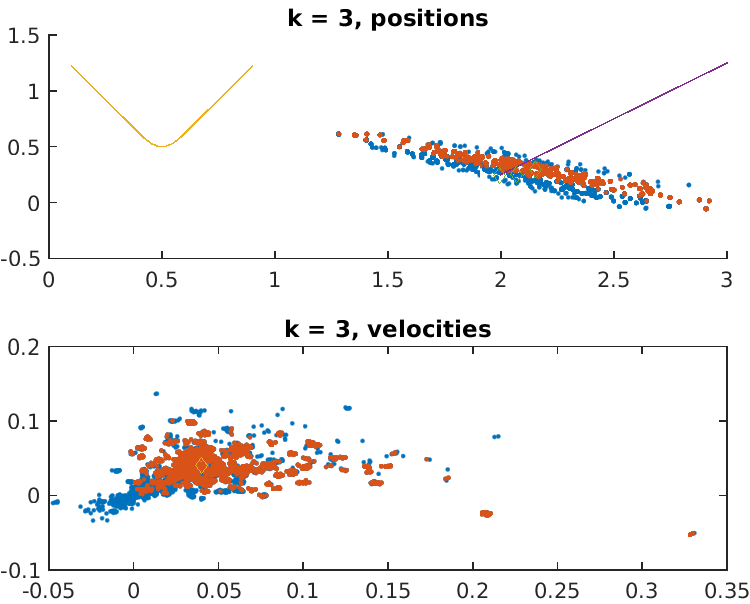
\includegraphics[width=0.98\textwidth]{img/q4_3.png}
	\end{minipage}%
	\begin{minipage}{.5\textwidth}
		 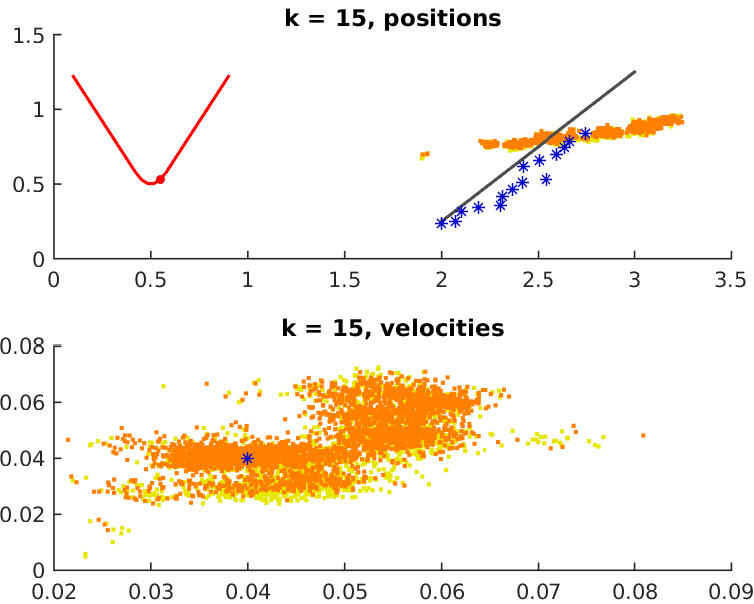
\includegraphics[width=0.98\textwidth]{img/q4_15.png}
	\end{minipage}
\end{center}
  \begin{center}
		 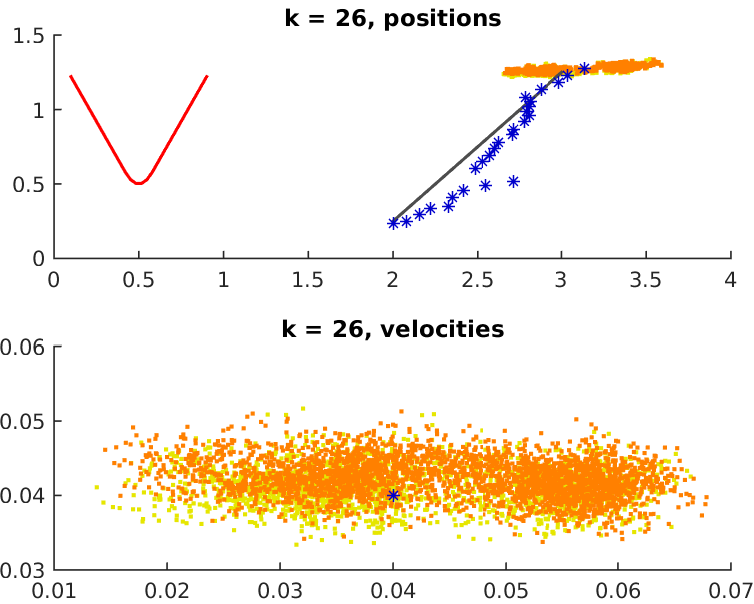
\includegraphics[width=0.5\textwidth]{img/q4_26.png}
\end{center}
  


\chapter{Improving the results using a post-regularised sequential
Monte Carlo method}
\section*{Code}

\section*{Results}
Results for question 5, part 1:
\begin{center}
   \includegraphics[width=0.6\textwidth]{img/q51.eps}
\end{center}

Results for question 5, part 2:
\begin{center}
   \includegraphics[width=0.6\textwidth]{img/q52.eps}
\end{center}

\chapter{Question 6}



\newpage
\chapter*{Solving the submarine tracking problem}
\lstinputlisting{../matlab/q4q5.m}
\chapter*{Question 4}
\lstinputlisting{../matlab/plot_q4.m}
\chapter*{Question 5}
\lstinputlisting{../matlab/plot_q5.m}
\lstinputlisting{../matlab/gen_plot5.m}
\chapter*{Question 6}
\end{document}
